\documentclass[svgnames,11pt]{beamer}
\input{/home/tof/Documents/Cozy/latex-include/preambule_commun.tex}
\input{/home/tof/Documents/Cozy/latex-include/preambule_beamer.tex}
%\usepackage{pgfpages} \setbeameroption{show notes on second screen=left}
\author[]{Christophe Viroulaud}
\title{Arbre binaire - représentation\\Coupe du monde 2018}
\date{\framebox{\textbf{Algo 07}}}
%\logo{}
\institute{Terminale - NSI}

\begin{document}
\begin{frame}
    \titlepage
        \note{\fcolorbox{black}{red}{{\LARGE cm2018.zip + slides}}}
\end{frame}
\begin{frame}
    \frametitle{}

    La France a (brillamment) gagné la coupe du Monde de football 2018. Pour stocker le tableau des phases finales le site web \emph{lateam.fr} utilise une structure simple de données.


\end{frame}
\begin{frame}
    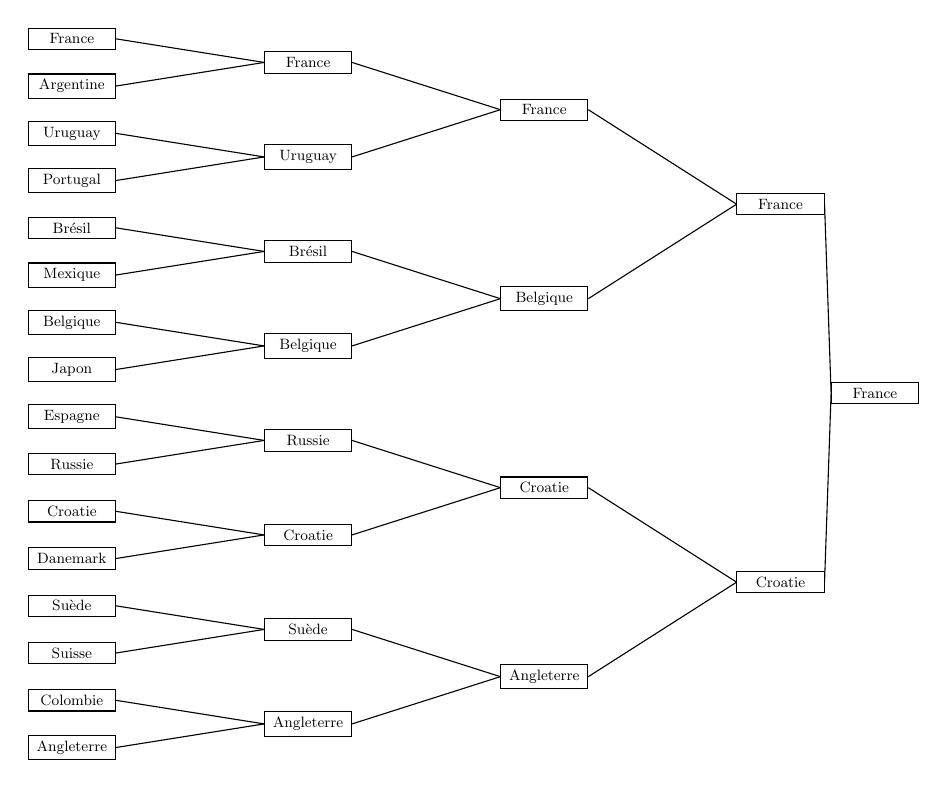
\begin{tikzpicture}[scale=0.6, transform shape,
            block/.style={
                    draw,
                    fill=white,
                    rectangle,
                    text width={width("Angleterre")},
                    align=center,
                    font=\small}]
        \node[block] (8-1) at (0,0) {Angleterre};
        \node[block] (8-2) at (0,1) {Colombie};
        \node[block] (8-3) at (0,2) {Suisse};
        \node[block] (8-4) at (0,3) {Suède};
        \node[block] (8-5) at (0,4) {Danemark};
        \node[block] (8-6) at (0,5) {Croatie};
        \node[block] (8-7) at (0,6) {Russie};
        \node[block] (8-8) at (0,7) {Espagne};
        \node[block] (8-9) at (0,8) {Japon};
        \node[block] (8-10) at (0,9) {Belgique};
        \node[block] (8-11) at (0,10) {Mexique};
        \node[block] (8-12) at (0,11) {Brésil};
        \node[block] (8-13) at (0,12) {Portugal};
        \node[block] (8-14) at (0,13) {Uruguay};
        \node[block] (8-15) at (0,14) {Argentine};
        \node[block] (8-16) at (0,15) {France};

        \node[block] (4-1) at (5,0.5) {Angleterre};
        \node[block] (4-2) at (5,2.5) {Suède};
        \node[block] (4-3) at (5,4.5) {Croatie};
        \node[block] (4-4) at (5,6.5) {Russie};
        \node[block] (4-5) at (5,8.5) {Belgique};
        \node[block] (4-6) at (5,10.5) {Brésil};
        \node[block] (4-7) at (5,12.5) {Uruguay};
        \node[block] (4-8) at (5,14.5) {France};

        \node[block] (2-1) at (10,1.5) {Angleterre};
        \node[block] (2-2) at (10,5.5) {Croatie};
        \node[block] (2-3) at (10,9.5) {Belgique};
        \node[block] (2-4) at (10,13.5) {France};

        \node[block] (1-1) at (15,3.5) {Croatie};
        \node[block] (1-2) at (15,11.5) {France};

        \node[block] (1) at (17,7.5) {France};

        \draw (8-1.east) -- (4-1.west);
        \draw (8-2.east) -- (4-1.west);
        \draw (8-3.east) -- (4-2.west);
        \draw (8-4.east) -- (4-2.west);
        \draw (8-5.east) -- (4-3.west);
        \draw (8-6.east) -- (4-3.west);
        \draw (8-7.east) -- (4-4.west);
        \draw (8-8.east) -- (4-4.west);
        \draw (8-9.east) -- (4-5.west);
        \draw (8-10.east) -- (4-5.west);
        \draw (8-11.east) -- (4-6.west);
        \draw (8-12.east) -- (4-6.west);
        \draw (8-13.east) -- (4-7.west);
        \draw (8-14.east) -- (4-7.west);
        \draw (8-15.east) -- (4-8.west);
        \draw (8-16.east) -- (4-8.west);

        \draw (4-1.east) -- (2-1.west);
        \draw (4-2.east) -- (2-1.west);
        \draw (4-3.east) -- (2-2.west);
        \draw (4-4.east) -- (2-2.west);
        \draw (4-5.east) -- (2-3.west);
        \draw (4-6.east) -- (2-3.west);
        \draw (4-7.east) -- (2-4.west);
        \draw (4-8.east) -- (2-4.west);

        \draw (2-1.east) -- (1-1.west);
        \draw (2-2.east) -- (1-1.west);
        \draw (2-3.east) -- (1-2.west);
        \draw (2-4.east) -- (1-2.west);

        \draw (1-1.east) -- (1.west);
        \draw (1-2.east) -- (1.west);

    \end{tikzpicture}

\end{frame}
\begin{frame}
    \frametitle{}

    \begin{framed}
        \centering Comment représenter simplement un arbre binaire en mémoire?
    \end{framed}

\end{frame}
\begin{frame}

    L'arbre binaire (figure \ref{arbre}) est numéroté en utilisant un parcours en largeur.
    \begin{center}
        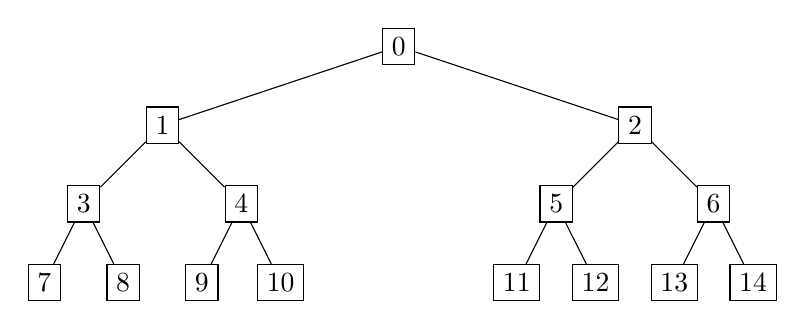
\begin{tikzpicture}
            \node[draw] (1) at (0,0) {0};
            \node[draw] (2) at (-3,-1) {1};
            \node[draw] (3) at (3,-1) {2};
            \node[draw] (4) at (-4,-2) {3};
            \node[draw] (5) at (-2,-2) {4};
            \node[draw] (6) at (2,-2) {5};
            \node[draw] (7) at (4,-2) {6};
            \node[draw] (8) at (-4.5,-3) {7};
            \node[draw] (9) at (-3.5,-3) {8};
            \node[draw] (10) at (-2.5,-3) {9};
            \node[draw] (11) at (-1.5,-3) {10};
            \node[draw] (12) at (1.5,-3) {11};
            \node[draw] (13) at (2.5,-3) {12};
            \node[draw] (14) at (3.5,-3) {13};
            \node[draw] (15) at (4.5,-3) {14};

            \draw (1) -- (2);
            \draw (1) -- (3);
            \draw (2) -- (4);
            \draw (2) -- (5);
            \draw (3) -- (6);
            \draw (3) -- (7);
            \draw (4) -- (8);
            \draw (4) -- (9);
            \draw (5) -- (10);
            \draw (5) -- (11);
            \draw (6) -- (12);
            \draw (6) -- (13);
            \draw (7) -- (14);
            \draw (7) -- (15);
        \end{tikzpicture}
        \captionof{figure}{Relation entre les indices}
        \label{arbre}
    \end{center}

\end{frame}
\begin{frame}
    \frametitle{}
    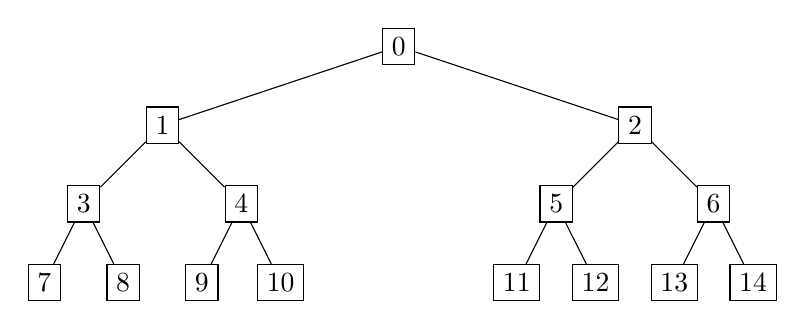
\begin{tikzpicture}
        \node[draw] (1) at (0,0) {0};
        \node[draw] (2) at (-3,-1) {1};
        \node[draw] (3) at (3,-1) {2};
        \node[draw] (4) at (-4,-2) {3};
        \node[draw] (5) at (-2,-2) {4};
        \node[draw] (6) at (2,-2) {5};
        \node[draw] (7) at (4,-2) {6};
        \node[draw] (8) at (-4.5,-3) {7};
        \node[draw] (9) at (-3.5,-3) {8};
        \node[draw] (10) at (-2.5,-3) {9};
        \node[draw] (11) at (-1.5,-3) {10};
        \node[draw] (12) at (1.5,-3) {11};
        \node[draw] (13) at (2.5,-3) {12};
        \node[draw] (14) at (3.5,-3) {13};
        \node[draw] (15) at (4.5,-3) {14};

        \draw (1) -- (2);
        \draw (1) -- (3);
        \draw (2) -- (4);
        \draw (2) -- (5);
        \draw (3) -- (6);
        \draw (3) -- (7);
        \draw (4) -- (8);
        \draw (4) -- (9);
        \draw (5) -- (10);
        \draw (5) -- (11);
        \draw (6) -- (12);
        \draw (6) -- (13);
        \draw (7) -- (14);
        \draw (7) -- (15);
    \end{tikzpicture}

    \vspace{1cm}

    Pour chaque nœud \emph{i} qui a des fils, on peut remarquer que:
    \begin{itemize}
        \item l'indice du fils gauche est $2×i+1$,
        \item l'indice du fils droit est $2×i+2$.
    \end{itemize}

\end{frame}
\begin{frame}
    \frametitle{}

    Un arbre binaire peut alors être stocké dans un simple tableau.
    \begin{center}
        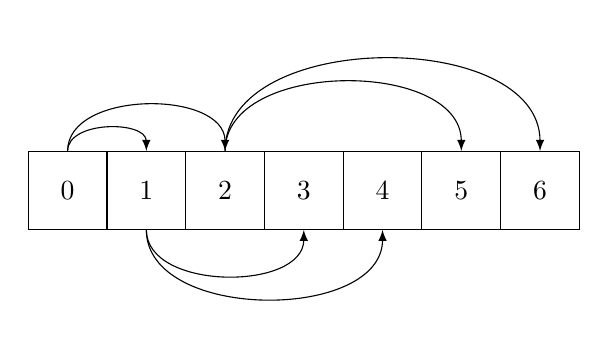
\begin{tikzpicture}
            \draw (0,0) grid (7,1);
            \node (0) at (0.5,0.5) {0};
            \node (1) at (1.5,0.5) {1};
            \node (2) at (2.5,0.5) {2};
            \node (3) at (3.5,0.5) {3};
            \node (4) at (4.5,0.5) {4};
            \node (5) at (5.5,0.5) {5};
            \node (5) at (6.5,0.5) {6};

            \draw[->,>=latex] (0.5,1) to[bend left=90] (1.5,1);
            \draw[->,>=latex] (0.5,1) to[bend left=90] (2.5,1);
            \draw[->,>=latex] (1.5,0) to[bend left=-90] (3.5,0);
            \draw[->,>=latex] (1.5,0) to[bend left=-90] (4.5,0);
            \draw[->,>=latex] (2.5,1) to[bend left=90] (5.5,1);
            \draw[->,>=latex] (2.5,1) to[bend left=90] (6.5,1);

        \end{tikzpicture}
        \captionof{code}{Un arbre binaire dans un tableau}
        \label{stocke}
    \end{center}
    \note{si arbre pas parfait certaines cases restent vides.
    }
\end{frame}
\begin{frame}
    \frametitle{}

    \begin{activite}
        \begin{enumerate}
            \item Télécharger le fichier \emph{cdm2018.zip} sur le site \url{https://cviroulaud.github.io} .
            \item Ouvrir le fichier \emph{cdm2018.json} et vérifier \emph{à la main} que le tableau représente bien l'arbre binaire des phases finales de la coupe du Monde 2018.
            \item Importer le \emph{json} dans un programme Python.
        \end{enumerate}
    \end{activite}

\end{frame}
\begin{frame}[fragile]
    \frametitle{Correction}

\begin{center}
\begin{lstlisting}[language=Python , basicstyle=\ttfamily\small, xleftmargin=2em, xrightmargin=2em]
f = open("cdm2018.json")
tab_cdm = json.load(f)
f.close()
\end{lstlisting}
\captionof{code}{Import}
\label{CODE}
\end{center}

\end{frame}
\begin{frame}
    \frametitle{}
\begin{center}
    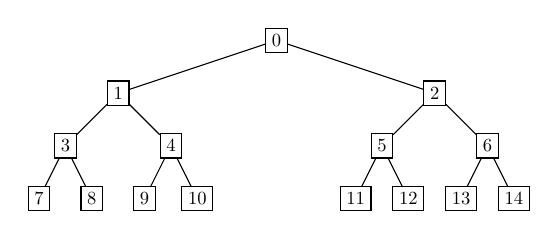
\begin{tikzpicture}[scale=0.67, transform shape]
        \node[draw] (1) at (0,0) {0};
        \node[draw] (2) at (-3,-1) {1};
        \node[draw] (3) at (3,-1) {2};
        \node[draw] (4) at (-4,-2) {3};
        \node[draw] (5) at (-2,-2) {4};
        \node[draw] (6) at (2,-2) {5};
        \node[draw] (7) at (4,-2) {6};
        \node[draw] (8) at (-4.5,-3) {7};
        \node[draw] (9) at (-3.5,-3) {8};
        \node[draw] (10) at (-2.5,-3) {9};
        \node[draw] (11) at (-1.5,-3) {10};
        \node[draw] (12) at (1.5,-3) {11};
        \node[draw] (13) at (2.5,-3) {12};
        \node[draw] (14) at (3.5,-3) {13};
        \node[draw] (15) at (4.5,-3) {14};

        \draw (1) -- (2);
        \draw (1) -- (3);
        \draw (2) -- (4);
        \draw (2) -- (5);
        \draw (3) -- (6);
        \draw (3) -- (7);
        \draw (4) -- (8);
        \draw (4) -- (9);
        \draw (5) -- (10);
        \draw (5) -- (11);
        \draw (6) -- (12);
        \draw (6) -- (13);
        \draw (7) -- (14);
        \draw (7) -- (15);
    \end{tikzpicture}
\end{center}

    \begin{activite}
        Considérons un arbre binaire parfait de hauteur \textbf{\texttt{h}} représenté par un tableau.
    \begin{enumerate}
        \item Quel est sa taille?
        \item Combien y-a-t-il de feuilles?
        \item Quel est l'indice de la feuille la plus à gauche?
        \item Écrire la fonction \textbf{\texttt{i\_feuille\_gauche(arbre: list) $\rightarrow$ int}} qui renvoie l'indice de la feuille la plus à gauche.
        \item Écrire alors la fonction \textbf{\texttt{get\_matchs(arbre: list) $\rightarrow$ list}} qui renvoie la liste des matchs de huitième de finale sous la forme d'un tableau de tuples.
    \end{enumerate}
    \end{activite}

\end{frame}
\begin{frame}
    \frametitle{Correction}

    \begin{itemize}
        \item La taille est $N=2^{(h+1)}-1$.
        \item Il y a $2^h$ feuilles.
        \item L'indice de la première feuille est $2^h-1$.
    \end{itemize}

\end{frame}
\begin{frame}[fragile]
    \frametitle{Correction}

\begin{center}
\begin{lstlisting}[language=Python , basicstyle=\ttfamily\small, xleftmargin=1em, xrightmargin=1em]
def i_feuille_gauche(arbre: list) -> int:
    """
    indice de la feuille la plus à gauche

    Args:
        arbre (list): arbre binaire parfait

    Returns:
        int: l'indice
    """
    i = 0
    while (2*i+1) < len(arbre):
        i = 2*i+1
    return i
\end{lstlisting}
\end{center}   

\end{frame}
\begin{frame}[fragile]

\begin{center}
\begin{lstlisting}[language=Python , basicstyle=\ttfamily\small, xleftmargin=1em, xrightmargin=1em]
def get_matchs(arbre: list) -> list:
    """
    huitième de finale

    Args:
        arbre (list): tableau du tournoi

    Returns:
        list: tableau de tuples
    """
    matchs = []
    i = i_feuille_gauche(arbre)
    while i < len(arbre):
        matchs.append((arbre[i], arbre[i+1]))
        i = i+2
    return matchs
\end{lstlisting}
\end{center}   

\end{frame}
\end{document}